%%%%%%%%%%%%%%%%%%%%%%%%%%%%%%%%%%%%%%%%%
% Beamer Presentation
% LaTeX Template
% Version 1.0 (10/11/12)
%
% This template has been downloaded from:
% http://www.LaTeXTemplates.com
%
% License:
% CC BY-NC-SA 3.0 (http://creativecommons.org/licenses/by-nc-sa/3.0/)
%
%%%%%%%%%%%%%%%%%%%%%%%%%%%%%%%%%%%%%%%%%

%----------------------------------------------------------------------------------------
%	PACKAGES AND THEMES
%----------------------------------------------------------------------------------------

\PassOptionsToPackage{prologue}{xcolor}
%\documentclass[notes,usenames,svgnames,dvipsnames,10pt]{beamer}
\documentclass[usenames,svgnames,dvipsnames,10pt]{beamer}

\usepackage{amsthm,amsmath,amssymb,amscd}
\usepackage{mathrsfs}

%\usepackage{CustomColors}

\definecolor{indiagreen}{rgb}{0.07,0.53,0.03}
\definecolor{GATechBlue}{rgb}{0.0,0.18823529411764706,0.3411764705882353}%{003057}
\definecolor{GATechGold}{rgb}{0.7019607843137254,0.6392156862745098,0.4117647058823529}%{B3A369​}
\definecolor{GATechBuzzGold}{rgb}{0.9176470588235294,0.6666666666666666,0.0}%{EAAA00}

\mode<presentation> {

% The Beamer class comes with a number of default slide themes
% which change the colors and layouts of slides. Below this is a list
% of all the themes, uncomment each in turn to see what they look like.

%\usetheme{default}
\usetheme{AnnArbor}
%\usetheme{Antibes}
%\usetheme{Bergen}
%\usetheme{Berkeley}
%\usetheme{Berlin}
%\usetheme{Boadilla}
%\usetheme{CambridgeUS}
%\usetheme{Copenhagen}
%\usetheme{Darmstadt}
%\usetheme{Dresden}
%\usetheme{Frankfurt}
%\usetheme{Goettingen}
%\usetheme{Hannover}
%\usetheme{Ilmenau}
%\usetheme{JuanLesPins}
%\usetheme{Luebeck}
%\usetheme{Madrid}
%\usetheme{Malmoe}
%\usetheme{Marburg}
%\usetheme{Montpellier}
%\usetheme{PaloAlto}
%\usetheme{Pittsburgh}
%\usetheme{Rochester}
%\usetheme{Singapore}
%\usetheme{Szeged}
%\usetheme{Warsaw}

% As well as themes, the Beamer class has a number of color themes
% for any slide theme. Uncomment each of these in turn to see how it
% changes the colors of your current slide theme.

%\usecolortheme{albatross}
%\usecolortheme{beaver}
%\usecolortheme{beetle}
%\usecolortheme{crane}
%\usecolortheme{dolphin}
%\usecolortheme{dove}
%\usecolortheme{fly}
%\usecolortheme{lily}
%\usecolortheme{orchid}
%\usecolortheme{rose}
%\usecolortheme{seagull}
%\usecolortheme{seahorse}
%\usecolortheme{whale}
%\usecolortheme{wolverine}

%\setbeamertemplate{footline} % To remove the footer line in all slides uncomment this line
%\setbeamertemplate{footline}[page number] % To replace the footer line in all slides with a simple slide count uncomment this line

%\setbeamertemplate{navigation symbols}{} % To remove the navigation symbols from the bottom of all slides uncomment this line

\setbeamercolor*{structure}{bg=GATechBlue,fg=GATechGold}

\setbeamercolor*{palette primary}{use=structure,fg=white,bg=structure.fg}
\setbeamercolor*{palette secondary}{use=structure,fg=white,bg=GATechGold!85!black}
\setbeamercolor*{palette tertiary}{use=structure,fg=white,bg=GATechGold!70!black}
\setbeamercolor*{palette quaternary}{fg=white,bg=GATechGold!65!white}

\setbeamercolor{frametitle}{bg=GATechBlue,fg=GATechBuzzGold}
\setbeamercolor*{titlelike}{bg=GATechBlue,fg=GATechBuzzGold}

\defbeamertemplate{itemize item}{bulletpoint}{\usebeamerfont*{itemize item enumitem}\raise1.05pt\hbox{\color{GATechGold!70!black}{$\blacktriangleright$}}}
\setbeamertemplate{items}[bulletpoint]

\setbeamercolor{section in toc}{fg=black}
\setbeamercolor{subsection in toc}{fg=black}

\setbeamercolor{bibliography item}{parent=palette primary}
\setbeamercolor{bibliography entry author}{fg=GATechBlue}
\setbeamercolor{bibliography entry title}{fg=GATechBlue}
\setbeamercolor{bibliography entry note}{fg=GATechBlue}

}

\usepackage{graphicx} % Allows including images
\usepackage{booktabs} % Allows the use of \toprule, \midrule and \bottomrule in tables
\usepackage{fancyvrb}
\usepackage{inconsolata}

\newcommand{\Iverson}[1]{\ensuremath{\left[#1\right]_{\delta}}} 

\DeclareMathOperator{\DGF}{DGF} 
\DeclareMathOperator{\ds}{ds} 
\DeclareMathOperator{\Id}{Id}
\DeclareMathOperator{\sq}{sq}

\newcommand{\ceiling}[1]{\ensuremath{\left\lceil #1 \right\rceil}} 
\newcommand{\ImportantMarker}{%\textcolor{GATechGold}{$\mathbf{\Leftarrow}$}\ 
                              \textcolor{GATechGold}{\textbf{[!! \underline{IMPORTANT} !!]}}}

\newcommand{\Floor}[2]{\ensuremath{\left\lfloor \frac{#1}{#2} \right\rfloor}}
\newcommand{\Ceiling}[2]{\ensuremath{\left\lceil \frac{#1}{#2} \right\rceil}}                              

\newcommand{\gkpSI}[2]{\ensuremath{\genfrac{\lbrack}{\rbrack}{0pt}{}{#1}{#2}}} 
\newcommand{\gkpSII}[2]{\ensuremath{\genfrac{\lbrace}{\rbrace}{0pt}{}{#1}{#2}}}

\newcommand{\TitleBoxed}[1]{
     \begin{beamercolorbox}[sep=8pt,center,shadow=true,rounded=true]{title}
          \usebeamerfont{title}#1\vskip 0.6cm\par%
     \end{beamercolorbox}
}

\usepackage{listings}
\definecolor{codeEnvBGColor}{rgb}{0.0,0.82,0.67}
\lstnewenvironment{code}{%
  \lstset{backgroundcolor=\color{codeEnvBGColor},
  frame=single,
  framerule=0pt,
  basicstyle=\ttfamily\scriptsize,
  breaklines=true,
  columns=fullflexible}}{}
\definecolor{pythonCodeEnvBGColor}{gray}{0.85}
\lstnewenvironment{pythoncode}{%
  \lstset{backgroundcolor=\color{pythonCodeEnvBGColor},
  frame=single,
  framerule=0pt,
  numbers=left,
  xleftmargin=1.9em,
  framexleftmargin=1.9em,
  stepnumber=1,
  basicstyle=\ttfamily\small,
  breaklines=true,
  language=Python}}{}
\lstnewenvironment{pythoncodesmall}{%
  \lstset{backgroundcolor=\color{pythonCodeEnvBGColor},
  frame=single,
  framerule=0pt,
  numbers=left,
  xleftmargin=3.5em,
  framexleftmargin=3.5em,
  stepnumber=1,
  basicstyle=\ttfamily\tiny,
  breaklines=true,
  language=Python}}{}

%\setbeamertemplate{note page}[plain]
\setbeamerfont{note page}{family*=pplx,size=\footnotesize} % Palatino for notes

%----------------------------------------------------------------------------------------
%	TITLE PAGE
%----------------------------------------------------------------------------------------

\title[Math 6307 Course Project]{
     Math 6307 Course Project: \\ Modern methods of exploration of numerical ODE solutions using Python3 
} 

\author{Maxie Dion Schmidt} % Your name
\institute[GA Tech] 
{
Georgia Institute of Technology \\ 
School of Mathematics \\ % Your institution for the title page
\medskip
\textit{maxieds@gmail.com} \\ 
\textit{mschmidt34@gatech.edu} \\ 
\medskip 
\url{http://people.math.gatech.edu/~mschmidt34/} \\ 
\url{https://github.com/maxieds/GATechMath6307ODEsCourseProject}
}
\date[November 9, 2021]{November 9, 2021 \\ {\small{\it (Last compiled with \LaTeX2e on \today)}}} % Date, can be changed to a custom date

\begin{document}

\begin{frame}
\titlepage % Print the title page as the first slide
%\note[item]{No notes for this page}
\end{frame} 

%----------------------------------------------------------------------------------------
%	PRESENTATION SLIDES
%----------------------------------------------------------------------------------------

%------------------------------------------------

\section{Overview and goals of the presentation} 

\begin{frame}
     \frametitle{Goals of the presentation}

\begin{itemize} 

     \item Explore options of modern packages for Python3 that facilitate exploring ODE (systems of ODEs) solutions numerically 
     \item Give a few examples of generic, \emph{\textbf{re-usable}} numerical methods for a toy 1D ODE problem
     \item Define and motivate the study of \emph{chaotic attractors} (corresponding to parameterized multidimensional systems of ODEs -- 
           typically 3D and 4D in a time variable, or 2D projections of such systems) 
     \item Show some particular experiment types for the \emph{R\"ossler attractor} that can be extended to other applications and use cases
     \item All source code, presentation materials and package install notes 
           for this project are freely available under the GPL-V3 at \\ 
           {\small{\url{https://github.com/maxieds/GATechMath6307ODEsCourseProject}}}

\end{itemize} 

\end{frame}

\section{Examples of solving ODEs in Python3}

\begin{frame}
\frametitle{Basic examples} 

\TitleBoxed{
     \Large{\centerline{Basic examples of solving ODEs in Python3}}
}

\end{frame}

\subsection{Setup: Model problem}

\begin{frame}
\frametitle{Setup: Defining a common model problem}

\begin{itemize} 

\item Typically we look at an IVP of the following form: \\ 
      $y^{\prime} = f(t, y), y(t_0) = y_0$
\item For the purposes of exploring our options in Python3, we will take a 
      special case of this problem type that is a \emph{stiff} ODE, or IVP that is highly 
      sensitive to the time mesh step size $h$ (facilitates comparison of the numerical methods)
\item The special case is defined simply as $y^{\prime} = -15y, y(0) = 1$ and hence has the 
      exact solution $y(t) = e^{-15t}$ for all $t \geq 0$ 
\item That is, $f(t, y) := -15y$ with $(t_0, y_0) := (0, 1)$
\item We will explore the solutions to this 1D linear (stiff) ODE system using the 
      following basic methods: 
      \begin{enumerate}
      \item Explicit forward Euler algorithm 
      \item Explicit Runge-Kutta (RK4) algorithm 
      \item Explicit multistep method: Adams-Bashforth (ABF-$3$) 
      %\item The \texttt{scipy.integration.odeint} function (adaptive integration of a vector-valued function) 
      %\item GEKKO python library ODE solver method (dynamic simultaneous simulation mode + solver)
      \end{enumerate} 

\end{itemize} 

\end{frame}

\subsection{Explicit forward Euler method}

\begin{frame}
\frametitle{Explicit forward Euler method}

\begin{itemize} 

\item Given an IVP: $y^{\prime} = f(t, y), y(t_0) = y_0$ 
\item The forward Euler method is an explicit method for iteratively 
      generating numerical solutions to this ODE provided that we can 
      evaluate $f$ clearly 
\item $\operatorname{LocalTruncationError} = O(h^2)$ (LTE at each step) 
\item if $f$ is Lipschitz, then $\operatorname{GlobalTruncationError} = O(h)$ 
       (depends on the function, or minimal Lipschitz constant, and the upper bound on the 
       time interval exponentially) 
\item $y_{n+1} = y_n + f(t_n, y_n) \left(t_{n+1} - t_n\right) = y_n + h \cdot f(t_n, y_n)$ \\ 
      $t_n = t_0 + nh$ for $n \in [0, N)$ and $N$ sufficiently large to guarantee convergence 
      to the solution 

\end{itemize} 

\end{frame}

\begin{frame}
\frametitle{Explicit forward Euler method -- Motivation}

\begin{itemize} 

\item \textbf{\emph{Key derivation}:} \\ 
      $y^{\prime}(t_0) \approx \frac{y(t_0+h)-y(t_0)}{h}$ ($\ast$), where 
      $y^{\prime} = f(t, y)$ $\implies$ $y(t_0+h)-y(t_0) \approx \int_{t_0}^{t_0+h} f(t, y(t)) dt$ 
\item Now we approximate the the RHS integral using a left-hand-endpoint Riemann sum ($n=1$ rectangle) to 
      obtain that $\int_{t_0}^{t_0+h} f(t, y(t)) dt \approx h \cdot f(t_0, y(t_0))$
\item Forward Euler is the simplest method using this line of reasoning 
\item Modifications can be given, including 
      taking $y^{\prime}\left(t + \frac{h}{2}\right) \approx \frac{y(t+h)-y(t)}{h}$ in place of ($\ast$) above, 
      leading to the \emph{midpoint method} 
\item Implicit backwards Euler forms another variant where we would take the RHS endpoint in the Riemann sum above

\end{itemize} 

\end{frame}

\begin{frame}[fragile]
\frametitle{Explicit foward Euler method (source code flavor)}

\begin{center}
\begin{pythoncode}
def ExplicitForwardEuler(ftyFunc, icPoint, solInterval, h):
    f = ftyFunc
    (t0, y0) = icPoint
    (solA, solB) = solInterval
    numGridPoints = math.floor(float((solB - solA) / h))
    tPoints = np.linspace(solA, solB, numGridPoints + 1)
    yPoints = [ y0 ]
    curYn = y0
    for n in range(0, numGridPoints):
        tn = tPoints[n]
        nextYn = curYn + f(tn, curYn) * h
        yPoints += [ nextYn ]
        curYn = nextYn
    # ... Matplotlib plotting code for the solution ... 
\end{pythoncode}
\end{center}

\end{frame}

\begin{frame}[fragile]
\frametitle{Explicit foward Euler method (results)}

\begin{center}
\begin{code}
(ipython) cd Examples/BasicNumericalODESolutionMethods
(ipython) run "ExplicitForwardEulerMethod.py"
\end{code}
\vskip -0.075cm
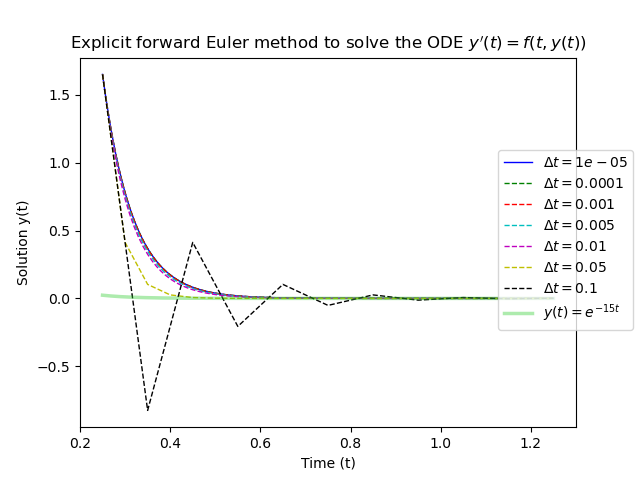
\includegraphics[height=0.76\textheight]{../Images/ExplicitForwardEuler-PlotOutput-StepSizeHComparison-v2.png}
\end{center}

\end{frame}

\subsection{Runge-Kutta (RK4) method}

\begin{frame}
\frametitle{Runge-Kutta (RK4) method}

\begin{itemize} 

\item Given an IVP: $y^{\prime} = f(t, y), y(t_0) = y_0$ 
\item $t_n = t_0 +h \cdot n$ (fixed / uniform step size)
\item $k_1 = f(t_n, y_n)$, $k_2 = f\left(t_n + \frac{h}{2}, y_n + \frac{k_1h}{2}\right)$, 
      $k_3 = f\left(t_n + \frac{h}{2}, y_n + \frac{k_2h}{2}\right)$, $k_4 = f\left(t_n + h, y_n + k_3h\right) $ 
\item $y_{n+1} = y_n + \frac{h}{6}\left(k_1 + 2k_2 + 2k_3 + k_4\right)$ (recursion to evaluate) 
\item Taking the weighted average at four slopes leads to more weight given to slopes closer to the midpoint 
      of each subinterval 
\item $\operatorname{LocalTruncationError} = O(h^5)$ and $\operatorname{GlobalTruncationError} = O(h^4)$ 
\item If $f$ does not depend on $y$, the RK4 is the same as \emph{Simpson's rule} 

\end{itemize} 

\end{frame}

\subsection{Runge-Kutta (RK4) method}

\begin{frame}
\frametitle{More general explicit Runge-Kutta methods}

\begin{itemize} 

\item The family of \emph{explicit RK methods} ($s$-stage) is paramterized by: \\ 
      $y_{n+1} = y_n + \sum\limits_{i=1}^{s} hb_ik_i$ where \\ 
      $k_1 = f(t_n, y_n)$ \\ 
      $k_2 = f(t_n + c_2h, y_n +h \cdot (a_{21}k_1))$ \\ 
      $k_3 = f(t_n + c_3h, y_n + h \cdot (a_{31}k_1 + a_{32}k_2))$ \\ 
      $\phantom{k_4}\cdots$ \\ 
      $k_s = f(t_n + c_sh, h \cdot(a_{s1}k_1 + a_{s2}k_2 + \cdots + a_{s,s-1}k_{s-1}))$. 
\item That is, the explicit RK method is completely determined by the parameters 
      $(a_{ij})_{1 \leq j < i \leq s}$, $(b_i)_{1 \leq i \leq s}$ and $(c_j)_{2 \leq j \leq s}$
\item We require \emph{consistency} insomuch as $\sum\limits_{i=1}^s b_i = 1$ 
\item A popular convention is to require that $\sum\limits_{j=1}^{i-1} a_{ij} = c_i$ for $i \in \{2,3,\ldots,s\}$ 
%\item \textbf{Variants:}  
%      There also exist second-order RK methods with two stages, adaptive RK methods, implicit RK methods 
%      (each has its own set of properties and advantages/disadvantages per use case, e.g., stability requirements)

\end{itemize} 

\end{frame}

\begin{frame}[fragile]
\frametitle{Runge-Kutta (RK4) method (results)}

\begin{center}
\begin{code}
(ipython) cd Examples/BasicNumericalODESolutionMethods
(ipython) run "RungeKuttaRK4Method.py"
\end{code}
\vskip -0.075cm
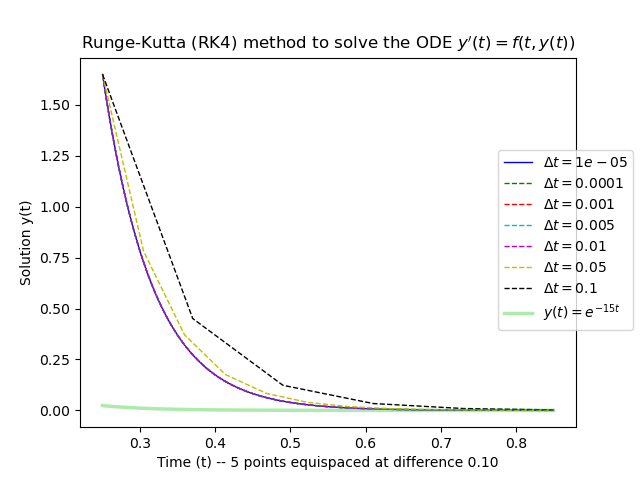
\includegraphics[height=0.76\textheight]{../Images/RungeKuttaRK4-PlotOutputs-StepSizeHComparison-v2.png}
\end{center}

\end{frame}

\subsection{Linear multistep solver method (general model and ABF-3)}

\begin{frame}
\frametitle{Step solver method -- Adams-Bashforth (ABF-$s$)}

\small 
\begin{itemize} 

\item The multistep ABF-$s$ ($s$-step) case: $a_{s-1}=-1$; $a_{s-2}=\cdots=a_0=0$
\item Lagrange's exact polynomial interpolation formula under this requirement: 
      $$p(t) = \sum\limits_{0 \leq j < s} \frac{(-1)^{s-j-1} f(t_{n+j}, y_{n+j})}{j! (s-j-1)! h^{s-1}} \times 
       \prod\limits_{\substack{0 \leq i < s \\ i \neq j}} (t-t_{n+i})$$ 
\item Approximations to initial conditions and foundation for building the numerical solutions: 
      $$y_{n} = y_{n-1} + \int\limits_{t_{n-1}}^{t_{n}} p(t) dt, \text{ for } n \in \{1, 2, \ldots, s-1\}$$ 
\item With $f(t_{n+j}, y_{n+j}) \mapsto p(t_{n+j})$, the ABF-$s$ method coefficient multipliers are: 
      $$b_{s-j-1} = \frac{(-1)^j}{j!(s-j-1)!} \times \int\limits_0^1 \prod\limits_{\substack{0 \leq i < s \\ i \neq j}} (u+i) du, 
       \text{ for } j \in \{0,1,\ldots,s-1\}$$ 
\item Recursion in the ABF-3 method: 
      $$y_{n+3} = y_{n+2} + h\left(\frac{23}{12}f(t_{n+2},y_{n+2}) - \frac{4}{3} f(t_{n+1},y_{n+1}) + \frac{5}{12} f(t_n, y_n)\right)$$ 

\end{itemize} 

\end{frame}

\begin{frame}[fragile]
\frametitle{Step solver method -- ABF3 (source code flavor)}

\begin{center}
\begin{pythoncodesmall}
def LagrangePolynomialInterpolation(ftyFunc, numStepsS, prevYPoints, t0, h, n):
    f             = ftyFunc
    s             = numStepsS 
    yPoints       = prevYPoints
    tDiffProdFunc = lambda t, j: reduce(operator.mul, [ t - (t0 + h * (n + i)) if i != j else 1 for i in range(0, s) ])
    ptFunc        = lambda t: sum([ (-1)**(s-j-1) * f(t0 + h * (n + j), yPoints[n+j]) / factorial(j) / \
                                    factorial(s-j-1) / (h**(s-1)) * tDiffProdFunc(t, j) \
                                    for j in range(0, n + len(yPoints)) ])
    nextYPoints   = []
    lastYPoint    = prevYPoints[-1]
    for sidx in range(0, s):
        tnpim1 = t0 + h * (n + sidx - 1)
        tnpi = t0 + h * (n + sidx)
        ynpi = lastYPoint + sympy.integrate(ptFunc(tvar), (tvar, tnpim1, tnpi))
        yPoints += [ ynpi ]
        nextYPoints += [ ynpi ]
        lastYPoint = ynpi
    return nextYPoints
def AdamsBashforthABF3(ftyFunc, icPoint, solInterval, h):
    f             = ftyFunc
    s             = 3
    (t0, y0)      = icPoint
    (solA, solB)  = solInterval
    numGridPoints = math.floor(float((solB - solA) / h))
    tPoints       = np.linspace(solA, solB, numGridPoints + 1)
    yPoints       = [ y0 ] + LagrangePolynomialInterpolation(f, s-1, [ y0 ], t0, h, n=0)
    curYn         = y0
    for n in range(0, numGridPoints + 1 - s):
        tn2, tn1, tn = tPoints[n+2], tPoints[n+1], tPoints[n]
        yn2, yn1, yn = yPoints[n+2], yPoints[n+1], yPoints[n]
        fn2, fn1, fn = f(tn2, yn2), f(tn1, yn1), f(tn, yn)
        nextYn = yn2 + h * (23.0 / 12.0 * fn2 - 4.0 / 3.0 * fn1 + 5.0 / 12.0 * fn)
        yPoints += [ nextYn ]
\end{pythoncodesmall}
\end{center}

\end{frame}

\begin{frame}[fragile]
\frametitle{Step solver method -- ABF3 (results)}

\begin{center}
\begin{code}
(ipython) cd Examples/BasicNumericalODESolutionMethods
(ipython) run "ABF3StepSolverMethod.py"
\end{code}
\vskip -0.205cm
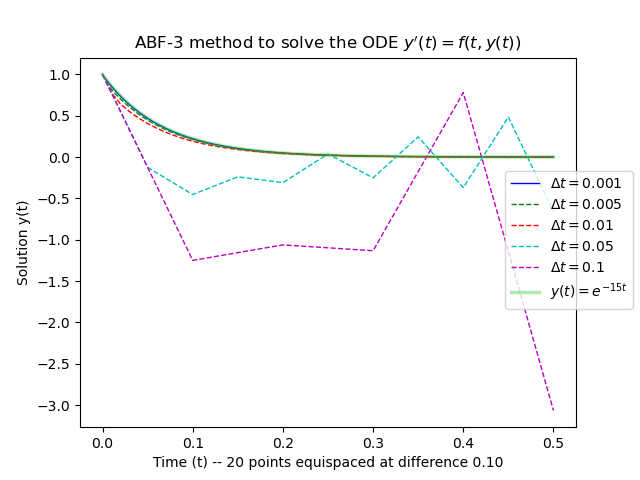
\includegraphics[height=0.76\textheight]{../Images/ABF3MultistepMethodResults-StepSizeHComparison-v2.png}
\end{center}

\end{frame}

\section{Chaotic Attractors} 

\begin{frame}
\frametitle{Key applications for numerical exploration} 

\TitleBoxed{
     \huge{\centerline{Chaotic attractors}}
}

\end{frame}

\begin{frame}
\frametitle{Definitions and motivation}

\begin{itemize} 
 
\item When considering dynamical systems, an \emph{attractor} is a set of states (orbits) towards which a system (of ODE solutions) 
      tends to evolve
\item System values within some small range of the \emph{attractor} set stay close even if perturbed slightly 
      (e.g., by slightly shifting an ODE initial condition) 
\item A \emph{chaotic attractor} is correspondingly an attractor admitting system that exhibit apparently randomized behavior and 
      disorderly irregularities in form 
\item Systems that form a \emph{chaotic attractor} type are highly sensitive to initial conditions 

\end{itemize} 

\end{frame}

\section{The R\"ossler Attractor} 

\subsection{Definitions} 

\begin{frame}
\frametitle{Definition of the R\"ossler attractor problem}

\begin{itemize} 

\item We will focus on numerical exploration of the \emph{R\"ossler attractor} system 
\item Non-linear 3D systems of ODEs determined by parameters $(a, b, c) \in \mathbb{R}^3$ 
\item Precise system: $(x^{\prime}, y^{\prime}, z^{\prime}) = (-y-z, x+ay, b + z(x-c))$ 
\item R\"ossler famously studied the ``classic'' case with $(a, b, c) := (0.2, 0.2, 5.7)$ 
      (important characteristic properties of other parameter special cases are known) 
\item Often times to simplify considerations, we consider a projection of the system corresponding to 
      setting one of the $XYZ$-components to zero, e.g., the projection in the $XY$-plane seen by setting 
      $z := 0$ 

\end{itemize} 

\end{frame}

\subsection{Numerical exploration of solutions} 

\begin{frame}[fragile]
\frametitle{Exploring the classical parameter solution}

\begin{center}
\vskip -0.5cm
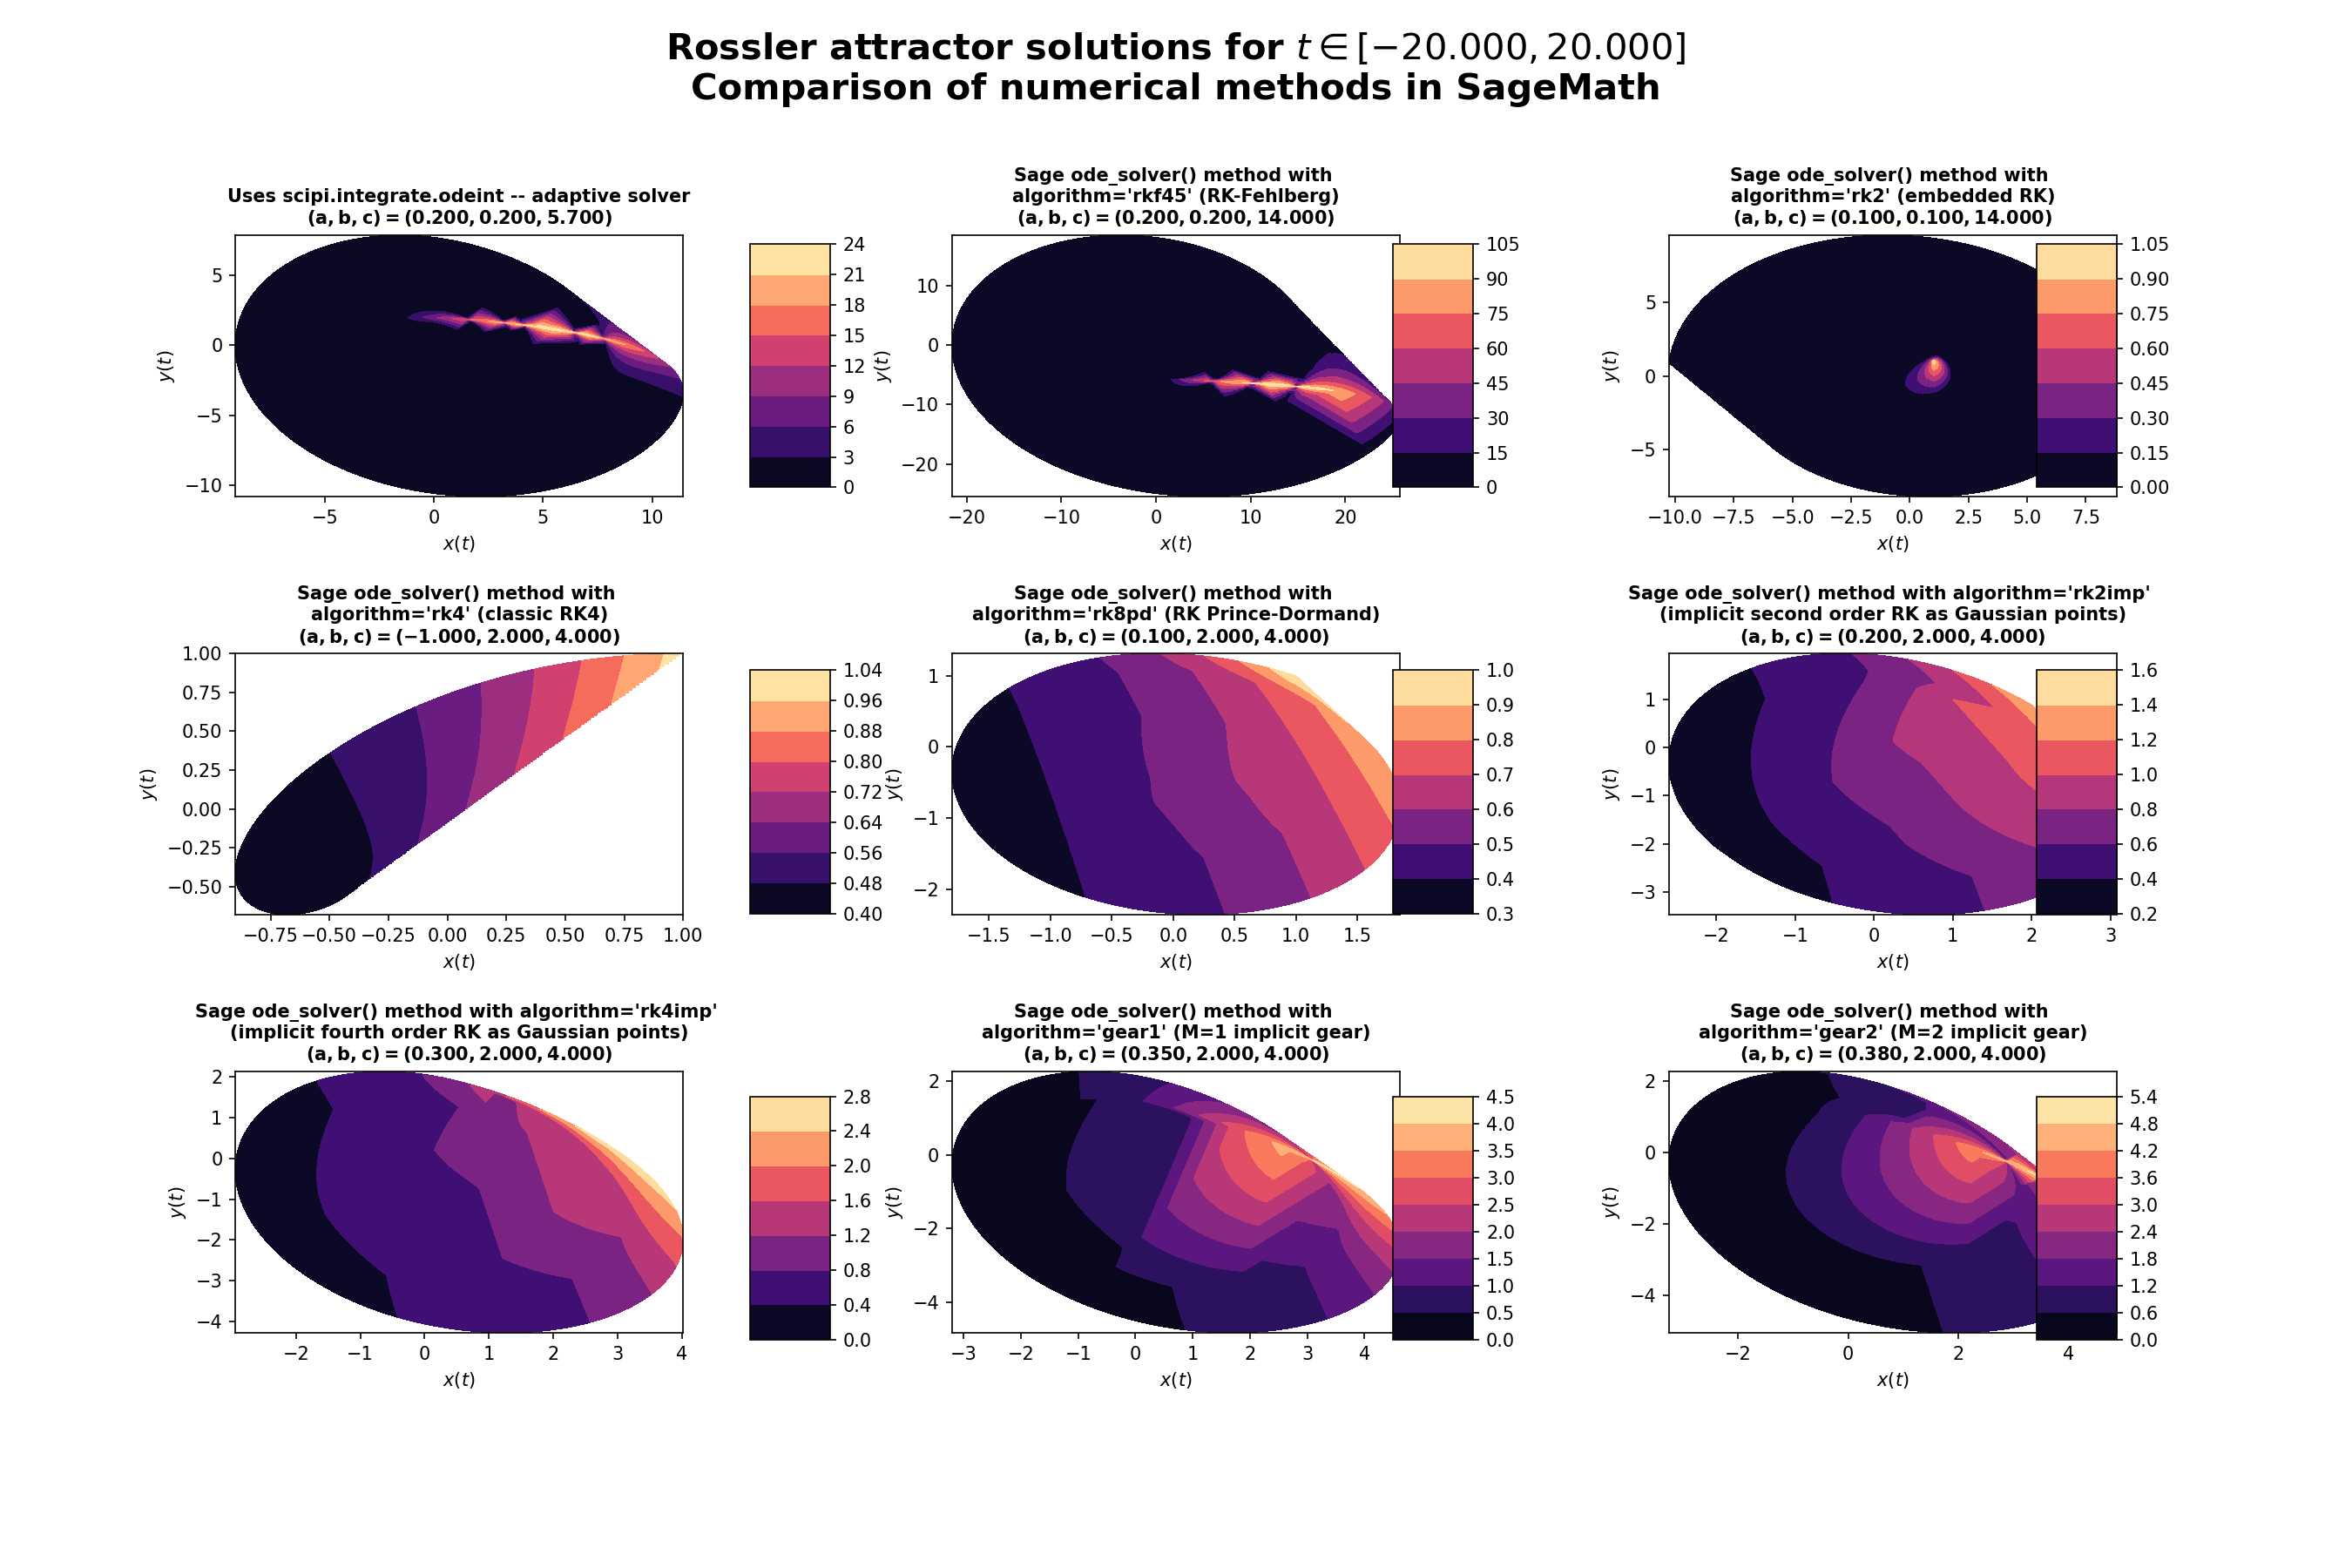
\includegraphics[height=0.92\textheight]{../Images/RosslerAttractorSage3DSolvers-2021-10-29-073902.png}
\end{center}

\end{frame}

\begin{frame}[fragile]
\frametitle{Exploring the classical parameter solution}

\begin{center}
\vskip -0.5cm
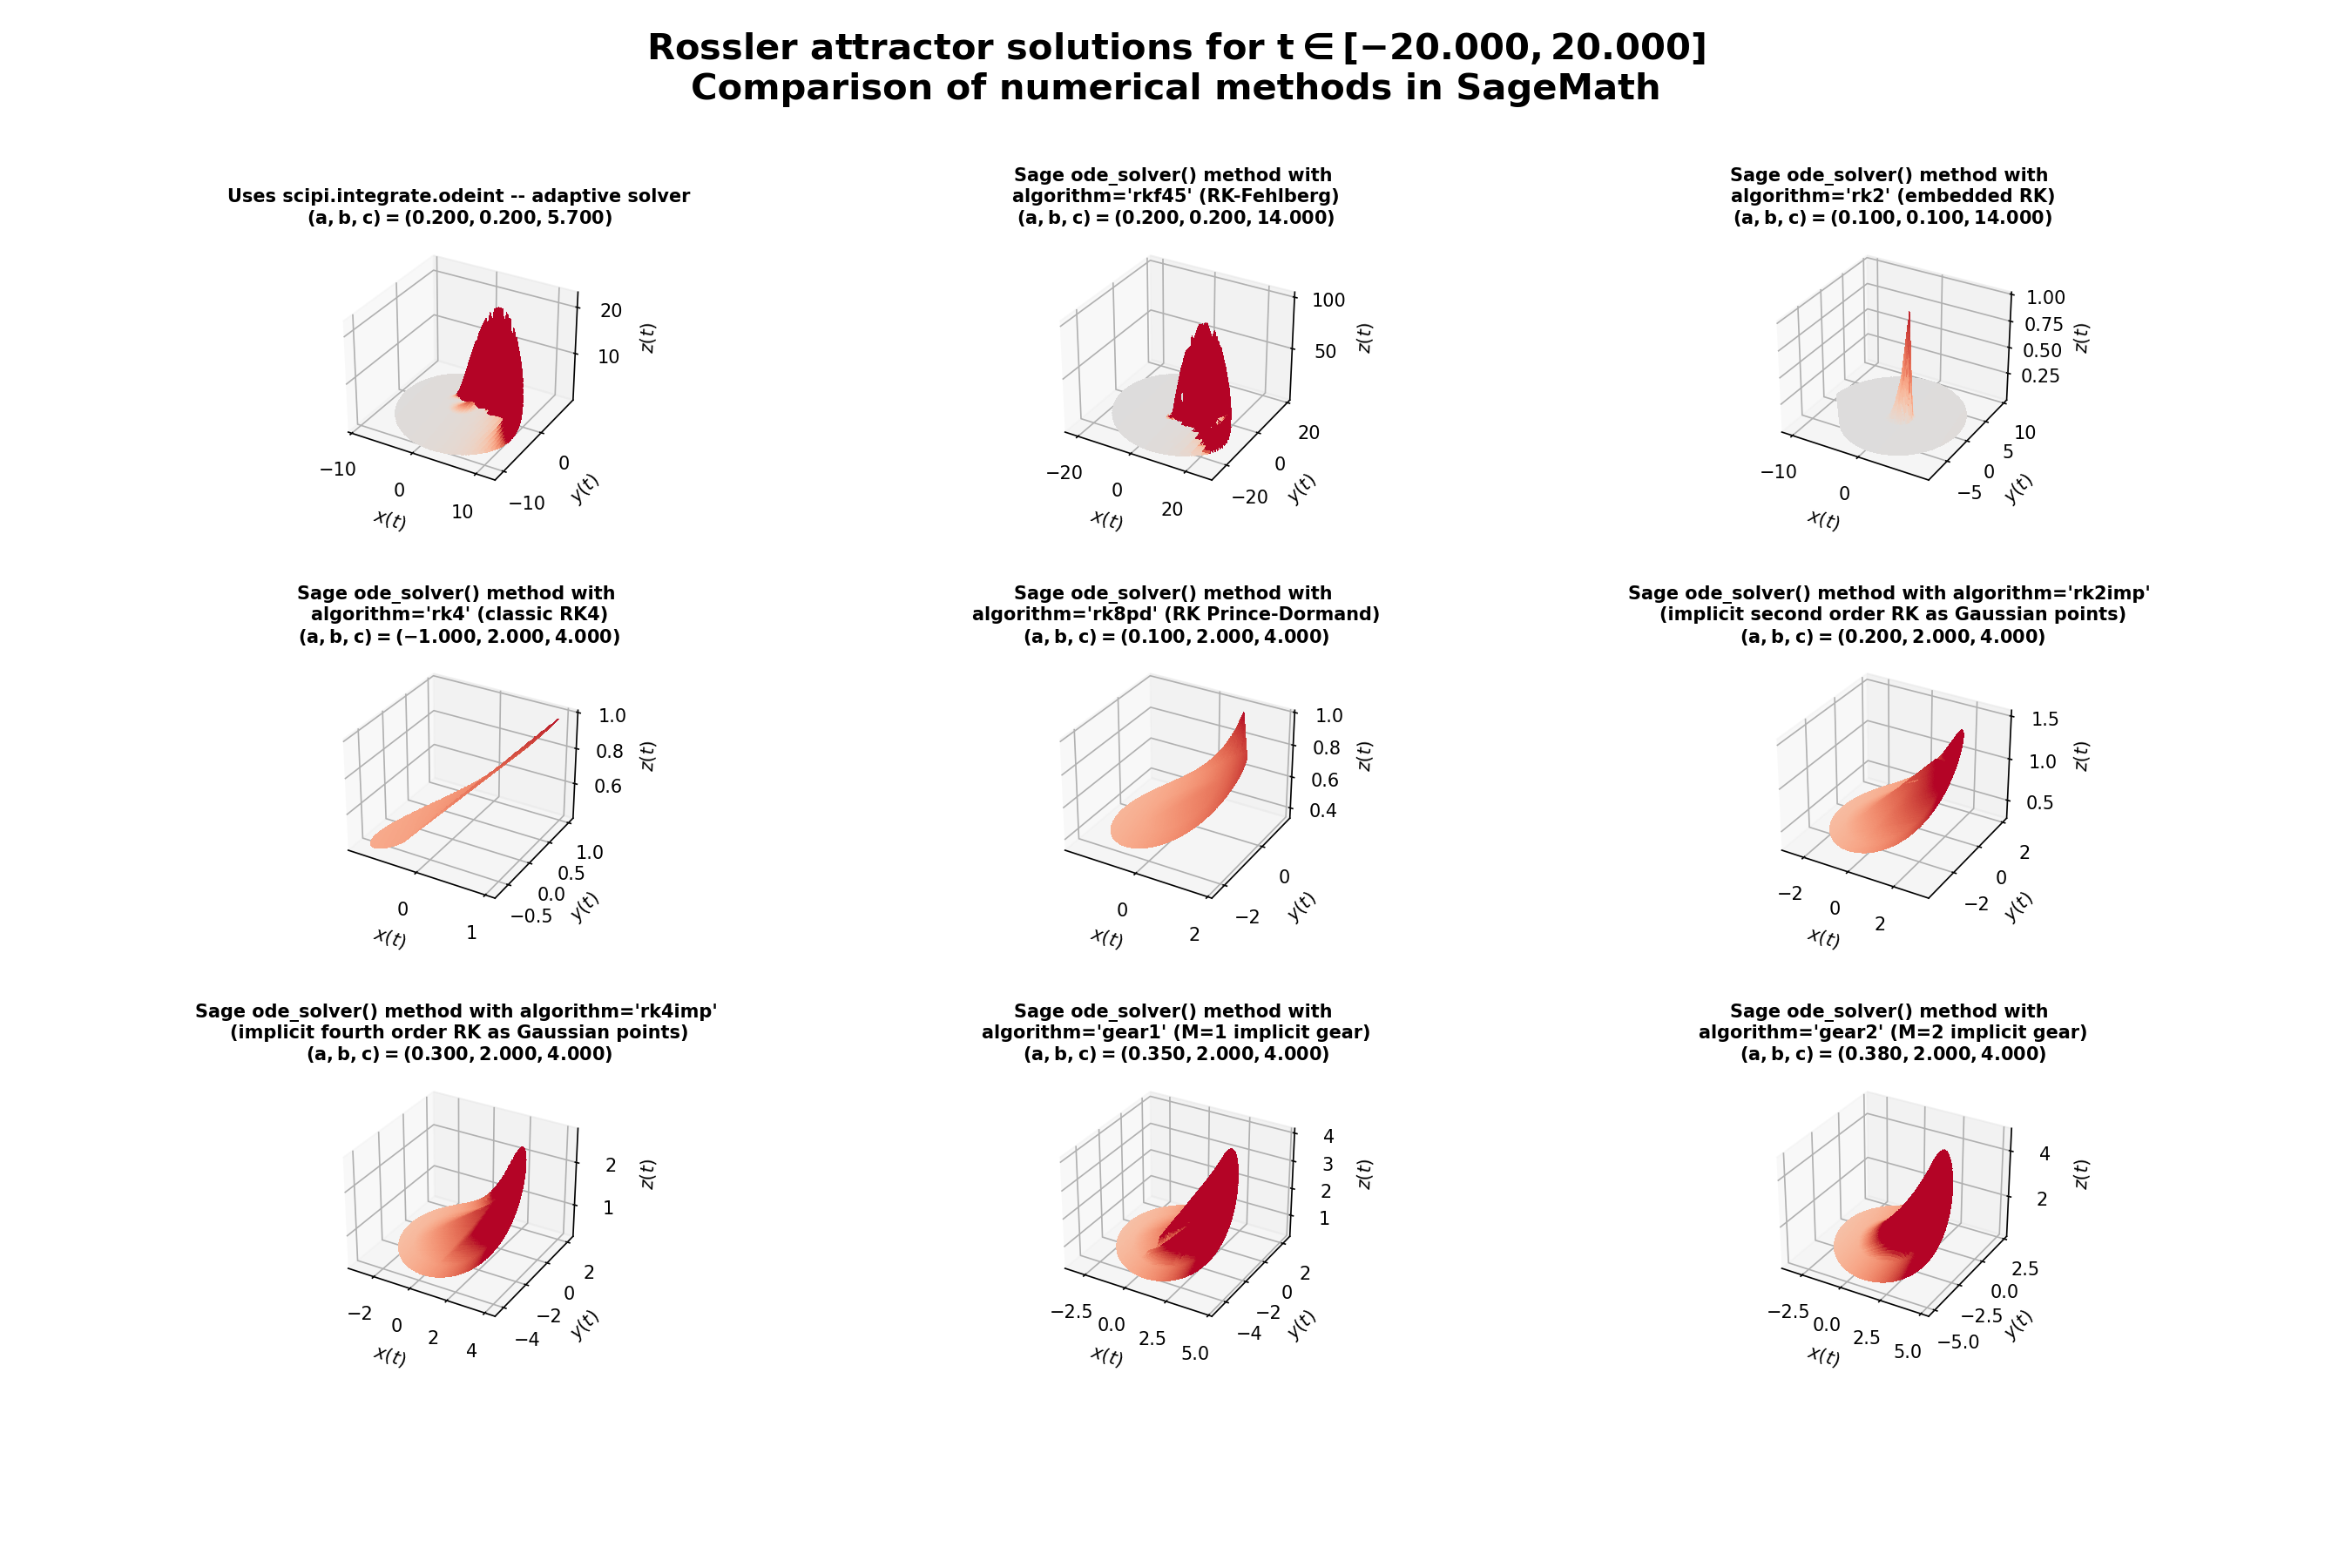
\includegraphics[height=0.92\textheight]{../Images/RosslerAttractorSage3DSolvers-2021-10-29-081641.png}
\end{center}

\end{frame}

\section{Concluding Remarks} 

\begin{frame}
\frametitle{Concluding remarks and discussion} 

     \Huge{\centerline{The End}}\smallskip
     \Large{\centerline{Questions?}}\smallskip
     \Large{\centerline{Comments?}}\smallskip
     \Large{\centerline{Feedback?}}\bigskip
     \Huge{\centerline{Thank you for attending!}} 

\end{frame}

\begin{frame}[t,allowframebreaks] 
\frametitle{References} 

\footnotesize 
\begin{thebibliography}{10}

\bibitem{CHAOS-BOOK} 
K.~T.~Alligood, T.~D.~Sauer and J.~A.~Yorke. 
\emph{CHAOS: An introduction to dynamical systems} 
(cf.\ Chapter 6: \emph{Chaotic attractors}). 
Springer Textbooks in Mathematical Sciences, New York, 1997. 

\bibitem{WIKI-EULER-METHOD}
\emph{Euler method}. \url{https://en.wikipedia.org/wiki/Euler_method}

\bibitem{WIKI-LINEAR-MULTISTEP-METHOD} 
\emph{Linear multistep method}. \url{https://en.wikipedia.org/wiki/Linear_multistep_method} 

\bibitem{CATTR-SURVEY} 
C.~Robinson. \emph{What is a chaotic attractor?} 
\url{https://sites.math.northwestern.edu/~clark/publications/chaos.pdf} (2021)

\bibitem{WIKI-ROSSLER-ATTR}
\emph{R\"ossler attractor}. \url{https://en.wikipedia.org/wiki/R\%C3\%B6ssler_attractor}

\bibitem{WIKI-RK-METHOD} 
\emph{Runge-Kutta method}. \url{https://en.wikipedia.org/wiki/Runge-Kutta_methods} 

\end{thebibliography}

\end{frame} 

%----------------------------------------------------------------------------------------

\end{document} 

